\section{Filtrace}
\subsection{Elliptic filtry}
\begin{figure}[H] 
	\centering
	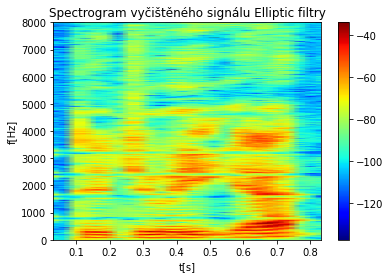
\includegraphics[scale=0.65,keepaspectratio]{Figure_20}
	\caption{Výkonový spektrogram vyčištěného signálu Elliptic filtry}
\end{figure}

\begin{figure}[H] 
	\centering
	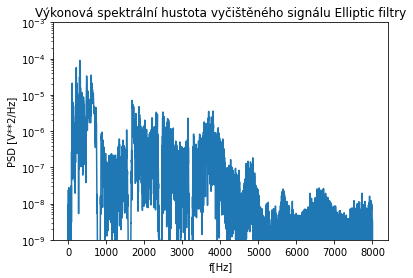
\includegraphics[scale=0.65,keepaspectratio]{Figure_21}
	\caption{Výkonová spektrální hustota vyčištěného signálu Elliptic filtry}
\end{figure}

\begin{landscape}
\begin{figure}[H] 
	\centering
	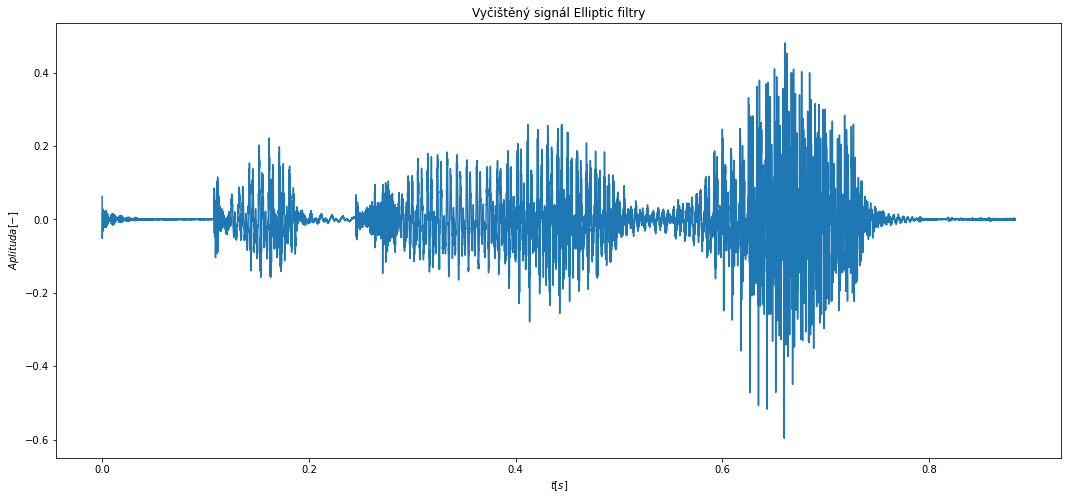
\includegraphics[scale=0.55,keepaspectratio]{Figure_23}
	\caption{Výsledný vyčištěný signál Elliptic filtry}
\end{figure}
\end{landscape}

\subsection{Butterworth filtry}
\begin{figure}[H] 
	\centering
	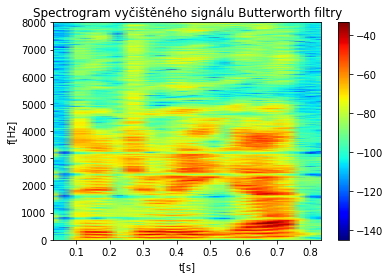
\includegraphics[scale=0.65,keepaspectratio]{Figure_27}
	\caption{Výkonový spektrogram vyčištěného signálu Butterworth filtry}
\end{figure}

\begin{figure}[H] 
	\centering
	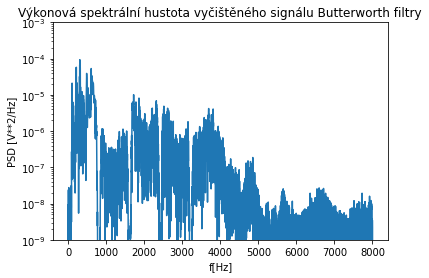
\includegraphics[scale=0.65,keepaspectratio]{Figure_28}
	\caption{Výkonová spektrální hustota vyčištěného signálu Butterworth filtry}
\end{figure}

\begin{landscape}
\begin{figure}[H] 
	\centering
	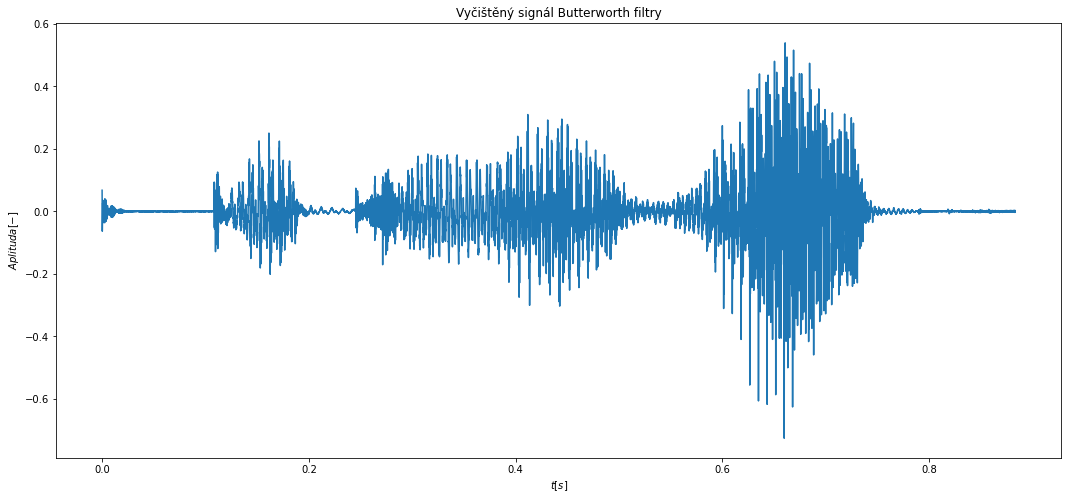
\includegraphics[scale=0.55,keepaspectratio]{Figure_29}
	\caption{Výsledný vyčištěný signál Butterworth filtry}
\end{figure}
\end{landscape}

\subsection{Shrnutí filtrace}
Vzhledem k tomu že se Butterworthův i Elliptic filtr chovali téměř identicky nebylo potřeba provádět čištění oběma.
Na výsledné číštění byl ale nakonec použit Elliptic filtr protože méně zkresluje signál na začátku a na konci.\\
Na spectrogramu vyčištěného signálu již nevidíme tak výrázné rušení i když nějaké rušení zde stále zůstalo. To může být způsobeno povahou rušení a nebo chováním filtru kde nemá na začátku ještě dostatek vzorků pro analýzu.
Můžeme vidět že i samotný signál je trochu zdeformovaný, což se dalo očekávat, jelikož část frekvenčního spektra tohoto signálu ležela ve stejné oblasti jako odstraňovaný šum.

\begin{landscape}
	\begin{figure}[H] 
		\centering
		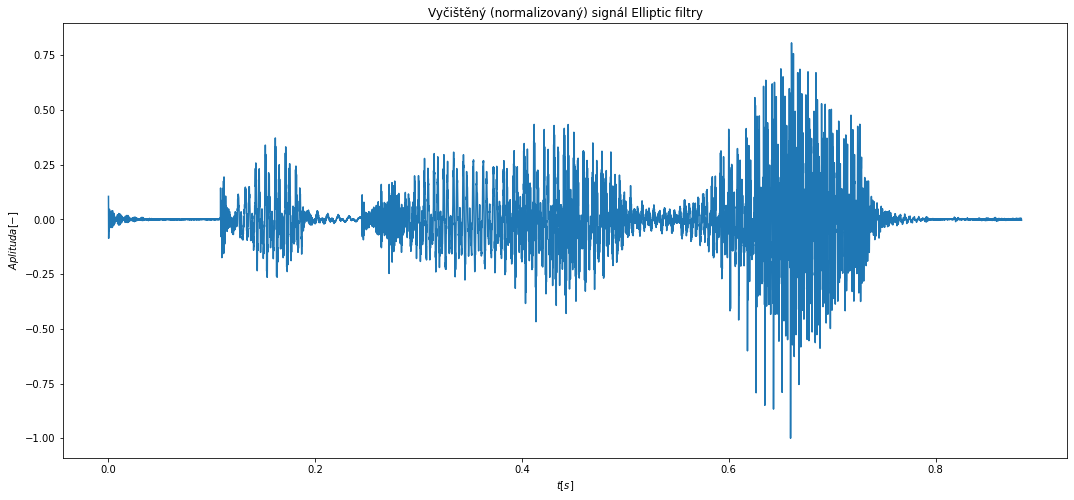
\includegraphics[scale=0.55,keepaspectratio]{Figure_30}
		\caption{Finální vyčištěný signál}
	\end{figure}
\end{landscape}